\documentclass[12pt]{article}
\usepackage[]{cite}
\usepackage{cmap}
\usepackage[T2A]{fontenc}
\usepackage[utf8]{inputenc}
\usepackage[english, russian]{babel}
\usepackage{amsmath, amsfonts,amssymb}
\usepackage{dsfont}
\usepackage{graphicx, epsfig}
\usepackage{subfig}
\usepackage{color}
\usepackage{comment}
\usepackage{algorithm}
\usepackage{algorithmic}
\usepackage{wrapfig}
\usepackage{url}



\newcommand\argmin{\mathop{\arg\min}}
\newcommand{\T}{^{\text{\tiny\sffamily\upshape\mdseries T}}}
\newcommand{\hchi}{\hat{\boldsymbol{\chi}}}
\newcommand{\hphi}{\hat{\boldsymbol{\varphi}}}
\newcommand{\bchi}{\boldsymbol{\chi}}
\newcommand{\A}{\mathcal{A}}
\newcommand{\B}{\mathcal{B}}
\newcommand{\x}{\mathbf{x}}
\newcommand{\hx}{\hat{x}}
\newcommand{\hy}{\hat{y}}
\newcommand{\M}{\mathcal{M}}
\newcommand{\N}{\mathcal{N}}
\newcommand{\R}{\mathbb{R}}
\newcommand{\p}{p(\cdot)}
\newcommand{\q}{q(\cdot)}
\newcommand{\uu}{\mathbf{u}}
\newcommand{\vv}{\boldsymbol{v}}

\DeclareMathOperator*{\argmax}{argmax}


\renewcommand{\baselinestretch}{1}

\newtheorem{Th}{Теорема}
\newtheorem{Def}{Определение}
\newenvironment{Proof} % имя окружения
    {\par\noindent{\bf Доказательство.}} % команды для \begin
    {\hfill$\scriptstyle\blacksquare$} % команды для \end
\newtheorem{Assumption}{Предположение}
\newtheorem{Corollary}{Следствие}

\textheight=24cm % высота текста
\textwidth=16cm % ширина текста
\oddsidemargin=0pt % отступ от левого края
\topmargin=-1.5cm % отступ от верхнего края
\parindent=24pt % абзацный отступ
\parskip=0pt % интервал между абзацами
\tolerance=2000 % терпимость к "жидким" строкам
\flushbottom % выравнивание высоты страниц

\graphicspath{ {./fig/} }



\begin{document}

\thispagestyle{empty}
\begin{center}
    \sc
        Министерство образования и науки Российской Федерации\\
        Московский физико-технический институт
        {\rm(государственный университет)}\\
        Физтех-школа прикладной математики и информатики\\
        Кафедра <<Интеллектуальные системы>>\\[35mm]
    \rm\large
        Панченко Святослав Константинович\\[10mm]
    \bf\Large
		Билинейность геометрического произведения для решения задачи декодирования \\[10mm]
    \rm\normalsize
        03.04.01 --- Прикладные физика и математика\\[10mm]
    \sc
        Выпускная квалификационная работа магистра\\[10mm]
\end{center}
\hfill\parbox{80mm}{
    \begin{flushleft}
    \bf
        Научный руководитель:\\
    \rm
        д.ф.-м.н. Стрижов Вадим Викторович\\[5cm]
    \end{flushleft}
}
\begin{center}
    Москва\\
    2022
\end{center}


\newpage
\tableofcontents
\newpage


\begin{abstract}
    Рассмотрена задача декодирования сигналов, представленных в виде синхронизированных временных рядов. В регрессионной задаче восстановления значений целевого ряда по значениям исходного требуется снизить размерность описания исходного сигнала. Предлагается способ снижения размерности с помощью построения пространственно-временного представления предыстории сигнала в конформной геометрической алгебре. Такое построение опирается на свойство билинейности геометрического произведения алгебры. Искомое низкоразмерное представление в данном подходе получается из коэффициентов мультивектора алгебры, характеризующего последовательность значений временного ряда. Предложенный метод применяется в решении задачи декодирования сигналов электрокортикограмм для восстановления траектории конечности.
    
  \bigskip
  \textbf{Ключевые слова}: \emph{задача декодирования сигналов, снижение размерности, конформная геометрическая алгебра, геометрическое произведение, пространственно-временное представление.}
\end{abstract}

\newpage

%%%%%%%%%%%%%%%%%%%%%%%%%%%%%%%%%%%%%%%%%%%%%%%%%%%%%%%%%%%%%%%%%%%%%%%%%%%%%%%%%%%%%%%%%%%%%%%%%%%%%%%%%%%%%%%%%%%%%%%%%%%%%%%%%%

\section*{Введение}
\addcontentsline{toc}{section}{\protect\numberline{}Введение}

\paragraph{Актуальность темы.} 
Задача декодирования сигналов -- одна из важнейших в области анализа временных рядов. Различные её постановки -- регрессионная, авторегрессионная, общая -- способны описать широкий класс задач, связанных с рядами, примеры которых рассмотрены в работах \cite{Grootswagers2017, Bao2017}. Одним из способом извлечь из сигнала признаковое описание для регрессионной задачи является переход в траекторное, или фазовое, пространство ряда, элементом которого является совокупность последовательных во времени значений ряда заданной длины. Полученное при таком подходе признаковое описание, достаточно богатое для качественного предсказания, имеет слишком высокую размерность для практического применения. Отсюда возникает фундаментальная проблема снижения размерности в фазовом пространстве временного ряда, рассмотренная в \cite{ISACHENKO2019, Motrenko2018, Katrutsa2017}.

Требуется разработать метод снижения размерности фазовых представлений. Такой метод позволяет получить информативные низкоразмерные описания временных рядов, способные улучшить качество и значительно снизить сложность предсказательных моделей. Полученные при помощи этих методов  представления активно используются в самых разных прикладных задачах обработки и анализа сигналов. 

\paragraph{Существующие решения.} 

Один из подходов к решению данной задачи -- метод PLS (\textit{Partial Least Squares} или \textit{Projection to Latent Structures}), описанный, в частности, в работах \cite{Haenlein2004, Geladi1988}. В то время как метод главных компонент позволяет отыскать в пространстве значений исходного сигнала подпространство, проекция сигнала на которое имеет максимальную дисперсию, метод PLS осуществляет проектирование в новое пространство как исходного, так и целевого сигнала. Таким образом, ковариация между сигналами моделируется при помощи скрытых переменных.
\paragraph{}

Ещё один метод отбора признаков, т.е. частный случай методов снижения размерности, QPFS (\textit{Quadratic Programming Feature Selection}), впервые введённый в работе \cite{RodrguezLujn2010QuadraticPF} отбирает в регрессионной задаче некореллированные признаки, наиболее релевантные целевой переменной. Для указанного отбора предлагается минимизировать функционал, где в качестве переменной выступает вектор индикаторов выбранных признаков, после чего в возникающей задаче оптимизации производится линейная релаксация.


\paragraph{}
В смежных областях распространение получили методы, основанные на  пространственно-временном представлении данных, пригодные для широкого класса задач машинного обучения, в том числе связанных с анализом временных рядов. Примеры таких исследований можно найти в работах \cite{Thiruvengadam2020, Yuan2010, Hu201, Lasenby1998}. Такие методы основаны на теории сетей и алгебраической топологии, а вместо матричных представлений прибегают к описанию данных с помощью методов геометрической алгебры -- инструмента, обобщающего приёмы линейной алгебры для компактного и единообразного описания линейных подпространств и операторов.


\paragraph{Цель работы.} 

Целью работы является построение нелинейного метода снижения размерности в фазовом пространстве сигнала, заключающегося в формировании пространственно-временного представления ряда в геометрической алгебре. Предыстории исходного временного ряда предлагается сопоставить мультивектор конформной геометрической алгебры. Этот мультивектор выступает для отрезка сигнала в роли низкоразмерного информативного признакового описания для регрессионной задачи восстановления значений целевого ряда. Требования, предъявляемые к полученным при использовании метода мультивекторам:
\begin{itemize}
    \item[] \textbf{снижение размерности} относительно длины используемого отрезка временного ряда:
    \item[] \textbf{информативность} с точки зрения качества решения задачи декодирования сигналов с использованием полученного мультивекторного представления;
    \item[] \textbf{интерпретируемость} полученных мультивекторов как элементов конформной геометрической алгебры.
\end{itemize}


\paragraph{Новизна.} 

Предлагается, воспользовавшись аналогами пространственно-временных представлений, описанных в \cite{Thiruvengadam2020, Yuan2010}, построить информативные мультивекторные описания для задачи декодирования. При таком построении мы отказываемся от множества упрощений, допускаемых в вышеупомянутых работах и пользуемся свойстами конформной геометрической алгебры и геометрического произведения для получения уникального признакового описания, позволяющего осуществить высокоточное восстановление значений целевого сигнала.

\paragraph{Основные положения, выносимые на защиту.}
\begin{enumerate}
    \item Предлагается метод снижения размерности в задаче анализа сигналов в виде алгоритма построения мультивекторного описания представления предыстории исходного временного ряда.
    \item Подтверждается гипотеза о возможности построения мультивектора, являющегося информативным представлением элемента фазовой траектории сигнала.
    \item Полученный метод успешно применяется в прикладной задаче декодирования сигналов электрокортикограмм для предсказания координат конечности.
\end{enumerate}




\newpage
\section{Постановка задачи декодирования  в мультивекторном представлении}
\paragraph{}
В данном разделе формально ставится задача декодирования временных рядов. Демонстрируются общие положения геометрической алгебре и осуществляется переход к задаче поиска конформного мультивекторного представления предыстории ряда.

\subsection{Постановка задачи декодирования и её обобщения}
\paragraph{}
Поставим задачу восстановления регрессионной зависимости между синхронизированными сигналами, представленными в виде временных рядов, следуя общепринятым обозначениям в постановке задачи декодирования, позаимстовованным из \cite{Is2018}.
\paragraph{}
Рассмотрим случай одномерных рядов. Пусть имеется пара $\textbf{s}_x, \textbf{s}_y$ -- исходный и целевой сигналы, соответственно. Каждый из рядов $\textbf{s}$ представляет собой последовательность значений $[s_1, \dots, s_T]^\intercal$ в моменты времени $1, \dots, T$.
\paragraph{}
Символами $x_t := [\textbf{s}_x]_t \in \mathds{R}, y_t := [\textbf{s}_y]_t \in \mathds{R}$ обозначим \textit{временные представления} рядов  -- совокупность измерений сигналов в момент времени $t$. Далее, \textit{представление предыстории} размерности $h$ исходного сигнала $\textbf{s}_x$ в момент времени $t$ представляет собой последовательность временных представлений $\textbf{X}_{t,h} = [x_{t-h+1}, \dots, x_t]^\intercal \in \mathds{R}^h$. Наконец, \textit{представление горизонта прогнозирования} размерности $p$ целевого сигнала $\textbf{s}_y$ в момент времени $t$ -- это последовательность временных представлений $\textbf{Y}_{t,p} = [y_{t+1}, \dots, y_{t+p}]^\intercal \in \mathds{R}^p$.
\paragraph{}
Сформулируем задачу декодирования в регрессионной форме: требуется построить предсказательную модель $\textbf{f}^R_{\textbf{XY}}: \mathds{R}^h \rightarrow \mathds{R}^p$, которая по представлению предыстории исходного сигнала восстанавливает горизонт прогнозирования целевого сигнала в соответствующий момент времени.
\paragraph{}
Функция $\textbf{f}^R_{\textbf{XY}}$ выбирается из параметрического семейства: $$\textbf{f}^R_{\textbf{XY}}\Big(\textbf{X}_{t,h}  \Big) = \textbf{f}^R_{\textbf{XY}}\Big( \textbf{X}_{t,h}  |   \boldsymbol{\theta} \Big),$$ 
где оптимальное значение параметров $\boldsymbol{\theta}^*$ находится минимизацией некоторой функции ошибки:
$$ \hat{\textbf{Y}}_{t,p} =  \textbf{f}^R_{\textbf{XY}}\Big( \textbf{X}_{t,h}  |   \boldsymbol{\theta} \Big),$$
$$ \boldsymbol{\theta}^* = \argmin_{\boldsymbol{\theta}}\mathcal{L}\Big(\hat{\textbf{Y}}_{t,p}, \textbf{Y}_{t,p}  \Big).$$

\newpage
\paragraph{}
Отметим, что предыстория $\textbf{X}_{t,h}$ и горизонт прогнозирования $\textbf{Y}_{t,p}$ являются элементами траекторных, или фазовых, пространств рядов $\textbf{s}_x, \textbf{s}_y$ размерности $h$ и $p$ соответственно, поэтому можно считать, что функция $\textbf{f}^R_{\textbf{XY}}$ осуществляет отображение между фазовыми пространствами рядов, что проиллюстрировано на Рис. \ref{fig:time_series}.

\vspace{1cm}
\begin{figure}[h]
    %\captionsetup{labelformat=empty}
    \centering
    \includegraphics[width = 0.8\textwidth]{fig/Постановка.eps}
    \caption{Регрессионная постановка задачи декодирования. Слева: представление предыстории исходного сигнала и представление горизонта прогнозирования целевого сигнала. Справа: предсказательная модель $\textbf{f}$ как функция между фазовыми пространствами рядов.}
    \label{fig:time_series}
\end{figure}

\paragraph{}
Приведём альтернативные постановки задачи декодирования:
\begin{enumerate}
    \item Авторегрессионная задача:\\ построить предсказательную модель $\textbf{f}^{AR}_{\textbf{YY}}: \mathds{R}^h \rightarrow \mathds{R}^p$, которая по представлению предыстории сигнала восстанавливает горизонт прогнозирования того же сигнала:
   $$ \hat{\textbf{Y}}_{t,p} =  \textbf{f}^{AR}_{\textbf{YY}}\Big( \textbf{Y}_{t,h} \Big).$$
   \item Общая задача:\\
   построить предсказательную модель $\textbf{f}_{\textbf{XY}}: \mathds{R}^{h_1} \times \mathds{R}^{h_2} \rightarrow \mathds{R}^p$, которая по представлениям предысторий исходного и целевого сигналов восстанавливает горизонт прогнозирования целевого сигнала:
   $$ \hat{\textbf{Y}}_{t,p} =  \textbf{f}_{\textbf{XY}}\Big(\textbf{X}_{t,h_1} \textbf{Y}_{t,h_2} \Big).$$
\end{enumerate}
\paragraph{}
Задачу декодирования также можно обобщить на случай многомерных рядов $\mathcal{S}_x = \{\mathbf{s}_x^1, \dots, \mathbf{s}_x^m \}$, $\mathcal{S}_y = \{\mathbf{s}_y^1, \dots, \mathbf{s}_y^r \}$, в случае чего пространства предыстории и горизонта прогнозирования меняются с $\mathds{R}^h, \mathds{R}^p$ на $\mathds{R}^{h \times m}, \mathds{R}^{p \times r}$.

\newpage
\subsection{Переход от фазового представления к мультивекторному}\label{GA}
\paragraph{} Прежде чем осуществлять переход к новому низкоразмерному представлению предыстории ряда, формально определим \textit{геометрическую алгебру} и её элементы -- \textit{мультивекторы}.
\paragraph{}
\textit{Геометрическая алгебра}, или алгебра Клиффорда, -- это обобщение линейной алгебры, обеспечивающее единообразное, не зависящее от координат описание линейных подпространств и геометрических операторов как равноправных элементов алгебры, наряду с векторами и скалярами. Аксиоматика и свойства геометрической алгебры подробно обсуждаются в \cite{Eric, Dorst2007GeometricAF}, ниже кратко приводятся некоторые важные результаты.
\paragraph{}
Формально, геометрическая алгебра -- это множество $\mathcal{G}$ c определёнными на нём операциями, сложением и умножением (последняя носит название \textit{геометрическое произведение}). Это множество подчиняется следующему набору аксиом:
\begin{enumerate}
    \item[]\textbf{Аксиома 1}. $\mathcal{G}$ -- кольцо с единцией, т.е., в частности:
        \begin{enumerate}
            \item[1)] множество замкнуто относительно операций сложения и произведения;
            \item[2)] сложение и произведение ассоциативны;
            \item[3)] у обеих операций есть \textit{единичный} элемент ($0$ и $1$ соответственно);
            \item[4)] у каждого элемента есть обратный по сложению;
            \item[5)] сложение коммутативно;
            \item[6)] произведение дистрибутивно относительно сложения справа и слева.
        \end{enumerate}
        
    \item[]\textbf{Аксиома 2}. $\mathcal{G}$ содержит подмножество $\mathcal{G}_0$ -- поле характеристики $0$, содержащее единичные элементы алгебры по сложению и умножению: $0$ и $1$. \\Элементы $\mathcal{G}_0$ назовём $0$-векторами или \textit{скалярами}.
    
    \item[]\textbf{Аксиома 3}. $\mathcal{G}$ содержит подмножество $\mathcal{G}_1$, замкнутое относительно сложения, и для любых $\lambda \in \mathcal{G}_0, \mathbf{v}\in \mathcal{G}_1:$ $\lambda \mathbf{v} =  \mathbf{v} \lambda  \in \mathcal{G}_1$. \\ Таким образом, $\mathcal{G}_1$ представляет собой линейную алгебру внутри $\mathcal{G}$, с $\mathcal{G}_0$ в качестве поля скаляров. Элементы $\mathcal{G}_1$ назовём $1$-векторами или просто \textit{векторами}.
    
    \item[]\textbf{Аксиома 4}. Квадрат каждого вектора является скаляром.\\
    Эквивалентная формулировка: симметризованное геометрическое произведение пары векторов, также называющееся в геометрической алгбере \textit{внутренним произведением}, является скаляром:
    $$\text{для любых } \mathbf{a},\mathbf{b} \in \mathcal{G}_1: \quad \quad a \rfloor b :=  \frac{1}{2}\big( \mathbf{a}\mathbf{b} + \mathbf{b}\mathbf{a}\big) = \frac{1}{2}\big( (\mathbf{a} + \mathbf{b})^2 - \mathbf{a}^2 - \mathbf{b}^2 \big) \in \mathcal{G}_0.$$
    
    Теперь, пользуясь следствиями из аксиом, можно классифицировать оставшиеся элементы геометрической алгебры. Пусть $r > 1$: произведение $r$ попарно ортогональных векторов назовём \textit{простым} $r$-\textit{вектором} ($r$-\textit{blade}); конечную сумму таких элементов -- $r$-\textit{вектором}. Множество $r$-векторов обозначим $\mathcal{G}_r$. \\
    В силу Аксиомы 3, если $A \in \mathcal{G}_r$, то $\lambda A \in {G}_r$ для любого скаляра $\lambda$. Поэтому $\mathcal{G}_r$ образует линейное пространство для всех $r$, c $\mathcal{G}_0$ в качестве поля скаляров.
\item[]\textbf{Аксиома 5}.
      Если $\mathcal{G}_0 = \mathcal{G}_1$, то $\mathcal{G} = \mathcal{G}_0$. Иначе $\mathcal{G}$ есть прямая сумма $\mathcal{G}_r$. \\
    Аксиома утверждает, в частности, что каждый элемент $A \in \mathcal{G}$ единственным образом предствавим в виде конечной суммы 
    $$A = \sum_r A_r, \text{ где } A_r \in \mathcal{G}_r,$$
    т.е. $A$ либо является $r$-вектором для конкретного $r$, либо является конечной суммой $r$-векторов для разных $r$ (смешанным мультивектором). \\
    Произвольный элемент геометрической алгебры назовём просто \textit{мультивектором}.
    
\end{enumerate}

    Получим выражение для одной из наиболее интересных операций в геометрической алгебре. Рассмотрим для этого геометрическое произведение пары векторов $\mathbf{a}$ и $\mathbf{b}$:
    $$ \mathbf{a}\mathbf{b} = \frac{1}{2}\big(\mathbf{a}\mathbf{b} + \mathbf{b}\mathbf{a}\big) + \frac{1}{2}\big(\mathbf{a}\mathbf{b} - \mathbf{b}\mathbf{a}\big) = \mathbf{a} \rfloor \mathbf{b} + \mathbf{a} \wedge \mathbf{b},$$
    где антисимметричная часть 
    $$\mathbf{a} \wedge \mathbf{b} := \frac{1}{2}\big(\mathbf{a}\mathbf{b} - \mathbf{b}\mathbf{a}\big) $$
    называется \textit{внешним произведением}. Дадим ему интерпретацию.
    \begin{enumerate}
        \item Случай коллинеарных векторов: если $\mathbf{a} \parallel \mathbf{b}$, то $\mathbf{a}\mathbf{b} - \mathbf{b}\mathbf{a} = 0$, произведение $\mathbf{a}\mathbf{b}$ коммутирует и $ \mathbf{a}\mathbf{b} = \mathbf{a} \rfloor \mathbf{b}$. При этом $\mathbf{a} \wedge \mathbf{b} = 0$.
        \item Случай ортогональных векторов: если $\mathbf{a} \rfloor \mathbf{b} = 0$, то $\mathbf{a}\mathbf{b}$ является простым бивектором, произведение $\mathbf{a}\mathbf{b}$ антикоммутирует и $B := \mathbf{a}\mathbf{b} = \mathbf{a} \wedge \mathbf{b}$. При этом:
$$ B^2 = \mathbf{a}\mathbf{b}\mathbf{a}\mathbf{b} = - \mathbf{a}\mathbf{b}\mathbf{b}\mathbf{a} = - \mathbf{a}^2\mathbf{b}^2 \text{ -- скаляр.}$$
        \item Общий случай: Представим $\mathbf{b}$ в виде суммы $\mathbf{b}_{\parallel} + \mathbf{b}_{\bot}, \mathbf{b}_{\parallel} = \lambda \mathbf{a}$. Тогда
    $$\mathbf{a}\mathbf{b}  = \mathbf{a}\mathbf{b}_{\parallel} + \mathbf{a}\mathbf{b}_{\bot}  = \mathbf{a} \rfloor \mathbf{b}_{\parallel} + \mathbf{a} \wedge \mathbf{b}_{\bot} = \lambda \mathbf{a}^2 + \mathbf{a} \wedge \mathbf{b}_{\bot};$$
$$\text{к тому же, } \mathbf{a}\mathbf{b} = \mathbf{a} \rfloor \mathbf{b} + \mathbf{a} \wedge \mathbf{b}.$$
В силу единственности разложения (Акс. 5)
$$\mathbf{a} \wedge \mathbf{b} = \mathbf{a} \wedge \mathbf{b}_{\bot} \text{ -- бивектор,}$$ соответствующий ориентированному сегменту плоскости, $(\mathbf{a} \wedge \mathbf{b})^2 = - |\mathbf{a}|^2|\mathbf{b}|^2\sin(\boldsymbol{\theta})$
    \end{enumerate}

\begin{figure}[h]
    %\captionsetup{labelformat=empty}
    \centering
    \includegraphics[width = 0.85\textwidth]{fig/Внешнее_произведение.eps}
    \caption{Внешнее произведение векторов, иллюстрация. Слева: случай ортогональный векторов. Справа: общий случай.}
\end{figure}

\paragraph{}
Полученный результат можно обобщить следующим образом: пусть $\mathbf{a}_1, \dots, \mathbf{a}_r$ -- совокупность из $r$ линейно независимых векторов. Тогда их внешнее произведение 
$$ \mathbf{a}_1 \wedge \dots \wedge \mathbf{a}_r$$
является $r$-вектором алгебры и соответствует ориентированному $r$-мерному параллелепипеду в $\mathcal{G}_1$. Аналогично можно утверждать, что этот элемент алгебры соответствует $r$-мерному линейному подпространству $\mathcal{G}_1$, образованному линейной оболочкой совокупности векторов. Последнее утверждение стоит понимать в следующем смысле: любой другой базис в этом же линейном подпространстве $\mathbf{b}_1, \dots, \mathbf{b}_r$ своим внешним произведением определит такой же элемент геометрической алгебры, с точностью до скалярного множителя.
Если же совокупность $\mathbf{a}_1, \dots, \mathbf{a}_r$ не является линейно независимой, то их внешнее произведение окажется равным нулю. 
\paragraph{}
Таким образом, с помощью операции внешнего произведения в геометрической алгебре из линейно независимых векторов можно конструировать элементы, соответствующие линейным подпространствам. Отметим также, что операции внутреннего и внешнего произведения можно обобщить, определив и проинтрепретировав их действия на произвольную пару мультивекторов $\mathcal{G}$.
\paragraph{}
Выше было рассмотрено аксиоматическое задание геометрической алгебры. Удобно, однако, рассмотреть векторное пространство, оснащённое квадратичной формой, например, $(\mathds{R}^{p,q}, Q)$ -- пространство столбцов высоты $n = p+q$ с сигнатурой $(p,q)$. Такое пространство порождает соответствующую геометрическую алгебру $\mathcal{G}^{p,q}$, где подмножества $\mathcal{G}_0$, $\mathcal{G}_1$ естественным образом наследуются из исходного векторного пространства. Для окончательного задания осталось лишь сопоставить квадрату каждого вектора в алгебре скаляр -- это осуществляется с использованием квадратичной формы $Q$: 
$$ \text{для любых } \mathbf{a} \in \mathcal{G}_1, \quad \quad \mathbf{a}^2 = Q(\mathbf{a}).$$

\paragraph{}
Если базисом исходного пространства служила совокупность $\mathbf{e}_1, \dots, \mathbf{e}_n$, то базисом в $\mathcal{G}^{p,q}$ послужит объединение базисов $\mathcal{G}^{p,q}_r$ для всех $r = 1, \dots, n$:
\begin{itemize}
    \item[]базис в $\mathcal{G}_0$: $\{1\}$, размерность -- $1$;
    \item[]базис в $\mathcal{G}_1$: $\{\mathbf{e}_1, \dots, \mathbf{e}_n\}$, размерность -- $n$;
    \item[]базис в $\mathcal{G}_2$: $\{\mathbf{e}_1 \wedge \mathbf{e}_2, \mathbf{e}_1 \wedge \mathbf{e}_3, \dots,\mathbf{e}_{n-1} \wedge \mathbf{e}_n\}$, размерность -- $C_n^2 = \frac{n(n-1)}{2}$;
    \item[]...
    \item[]базис в $\mathcal{G}_n$: $\{\mathbf{e}_1 \wedge \mathbf{e}_2 \wedge \mathbf{e}_3 \wedge \dots \wedge \mathbf{e}_n\}$, размерность -- $1$.
    
\end{itemize}
Подпространство $\mathcal{G}^{p,q}_r$ имеет размерность $C_n^r$. Геометрическая алгебра $\mathcal{G}^{p,q}$ является, таким образом, линейным пространством размерности: $$\dim \mathcal{G}^{p,q} = \dim \mathcal{G}^{p,q}_0 \oplus \mathcal{G}^{p,q}_1 \oplus \dots \oplus \mathcal{G}^{p,q}_n = \sum_{r=0}^n \dim \mathcal{G}^{p,q}_r  = \sum_{r=0}^n C_n^r =  2^n,$$
где $n = p + q$.

\paragraph{}
В соответствии с Аксиомой 5, каждый элемент $A \in \mathcal{G}$ единственным образом предствавим в виде конечной суммы $A = \sum_r A_r, \text{ где } A_r \in \mathcal{G}_r.$ Введём в соответствии с этим корректно определённый оператор грейда степени $r$ -- проектор в подпространство $r$-векторов: 
$$\langle \ \rangle_r:\mathcal{G} \rightarrow \mathcal{G}_r, \quad \quad  \langle A \rangle_r := A_r.$$
Например, для мультивектора $A = 1 + a \wedge b + c \wedge d \wedge e \wedge f$ в алгебре над пространством размерности $n \geq 4$, в предположении о линейной независимости векторов $a, b$ и $c, d, e, f$
имеем:
$$ \langle A \rangle_0 = 1, \quad \langle A \rangle_2 = a \wedge b, \quad \langle A \rangle_4 = c \wedge d \wedge e \wedge f, \quad \langle A \rangle_r = 0 \text{ для } r =1, r= 3, r > 4.$$

\paragraph{}
Единичный базисный элемент подпространства $\mathcal{G}_n$ алгебры над пространством размерности $n$, имеющий вид $I = \mathbf{e}_1\mathbf{e}_2\dots \mathbf{e}_n$, называется элементом гиперобъёма пространства, или \text{псевдоскаляром}. Последнее название проистекает из-за сходства одномерных пространств $\mathcal{G}_0$ и $\mathcal{G}_n$: оба пространства являются одномерными, и все их элементы отличаются друг от друга не более чем на скалярный множитель.
\paragraph{}
С псевдоскаляром $I$ в геометрической алгебре связан важный объект -- дуальный элемент $A^*$:
$$ A^* = A \rfloor I^{-1} = AI^{-1}.$$
Элемент $A^*$ интерпретируется как обобщение ортогонального дополнения к $A$ в алгебре и в некоторых источниках обозначается $A^\bot$.

\newpage
\subsection{Свойства конформной геометрической алгебры}
\paragraph{} Интересующая нас алгебра -- это \textit{конформная геометрическая алгебра} над пространством $\mathds{R}^{4,1}$, обладающая рядом полезных свойств.

\paragraph{}
Конформная геометрическая алгебра (\textit{Conformal Geometric Algebra}, CGA) -- это геометрическая алгебра $\mathcal{G}^{p+1,q+1}$, в общем случае порождённая пространством $\mathds{R}^{p+1, q+1}$, элементы которой способны описывать действие преобразований в пространстве $\mathds{R}^{p, q}$ на различные геометрические объекты. Подробное изложение свойств CGA можно найти в работах \cite{Miller2013GeometricAA, Cliff, Sommer2001GeometricCW}.Рассмотрим классический случай трёхмерного евклидова пространства $\mathds{R}^3$, сигнатура $(p=3,q=0)$, и соответствующей конфорvной алгебры $\mathcal{G}^{4,1}$.
\paragraph{}
Основные характеристики CGA:
\begin{enumerate}
    \item Конформные преобразования в $\mathds{R}^{3}$, т.е. преобразования, сохраняющие углы, представляются в CGA с помощью двухстороннего оператора (sandwitching operator):
    $$ V = v_1v_2\dots v_s, \text{ -- геометрическое произведение обратимых В } \mathcal{G}^{4,1} \text{ векторов;}$$
    $$ X \mapsto VXV^{-1} \text{ для чётного s;} \quad \ \ $$
    $$ X \mapsto - VXV^{-1} \text{ для нечётного s.} $$
    
    Наиболее интересные представители конформных отображений в  $\mathds{R}^3$ -- повороты, трансляции, инверсии и растяжения. Каждому из этих классов преобразований соответсвует своё семейство мультивекторов CGA. 
    \item Геометрические объекты, такие как точки, прямые, сферы, плоскости приобретают естественные представления как элементы конформной алгебры.
\end{enumerate}

\paragraph{}
Для описания того, каким образом элементы $\mathcal{G}^{4,1}$ могут описывать объекты и преобразования в $\mathds{R}^3$, служит \textit{конформное вложение} $F$ -- инъективное отображение из $\mathds{R}^3$ в $\mathds{R}^{4,1}$. Оно задаётся следующим образом:
\begin{enumerate}
    \item Пусть $\{\mathbf{e}_1, \mathbf{e}_2, \mathbf{e}_3\}$ -- базис в пространстве $\mathds{R}^3$. Базис в $\mathds{R}^{4,1}$ формируется добавлением к предыдущему пары базисных векторов $\mathbf{e}_+$ И $\mathbf{e}_-$, ортогональных друг другу и каждому из $\mathbf{e}_i$. При этом результирующее пятимерное пространство оснащается квадратичной формой с сигнатурой $(4,1)$, так что в $\mathcal{G}^{4,1}$ $\mathbf{e}_+^2 = +1,$ $\mathbf{e}_-^2 = -1$.
    \item Осуществляется замена базиса: переход от $\{\mathbf{e}_1, \mathbf{e}_2, \mathbf{e}_3, \mathbf{e}_+, \mathbf{e}_-\}$ к $\{\mathbf{e}_1, \mathbf{e}_2, \mathbf{e}_3, \mathbf{e}_o, \mathbf{e}_{\infty}\}$. Здесь:
    \begin{itemize}
        \item[] $\mathbf{e}_o = \frac{1}{2}(\mathbf{e}_- - \mathbf{e}_+), \ \mathbf{e}_o^2 = 0;$
        \item[] $\mathbf{e}_{\infty} = \mathbf{e}_+ + \mathbf{e}_-, \quad \   \mathbf{e}_{\infty}^2 = 0.$
    \end{itemize}
    
    \item Тогда точке $\mathbf{x} \in \mathds{R}^3$ сопоставляется точка  $X \in \mathds{R}^{4,1}$, являющаяся одновременно и вектором-элементом алгебры $\mathcal{G}^{4,1}$ -- стандартная форма конформного образа точки:
    $$F:\mathds{R}^3 \rightarrow \mathds{R}^{4,1}, \quad \quad X: = F(\mathbf{x}) := \mathbf{x} + \frac{1}{2}||\mathbf{x}||_2^2 \mathbf{e}_{\infty} + \mathbf{e}_o.$$

    \end{enumerate}
    
    \paragraph{}
    На самом деле, конформное вложение задаёт \textit{однородную систему координат} для установления соответствия между элементами $\mathds{R}^3$ и $\mathds{R}^{4,1}$ в следующем смысле (\cite{Miller2013GeometricAA}): отметим, что квадрат конформного образа $X$ точки $\mathbf{x}$ равен нулю:
    $$ X^2 = \Big(\mathbf{x} + \frac{1}{2}\big(||\mathbf{x}||_2^2 - 1\big)\mathbf{e}_+ + \frac{1}{2}\big(||\mathbf{x}||_2^2 + 1\big)\mathbf{e}_-\Big)^2 = $$
    $$ = ||\mathbf{x}||_2^2 + \frac{1}{4}\big(||\mathbf{x}||_2^4 - 2||\mathbf{x}||_2^2 + 1\big) - \frac{1}{4}\big(||\mathbf{x}||_2^4 + 2||\mathbf{x}||_2^2 + 1\big) = 0.$$

\noindent
    Также равен нулю квадрат элемента $\alpha X$ для любого ненулевого скаляра $\alpha$. Конформное вложение предполагает, что все точки вида $\alpha X$ являются взвешенными (с весом $|\alpha|$) ориентированными (в соответствии со знаком $\alpha$) представлениями одной и той же точки $\mathbf{x} \in \mathds{R}^3$. Отображение из $\mathds{R}^3$ в $\mathbf{R}^{4,1}$, для определённости, строится таким образом, чтобы начало координат в $\mathds{R}^3$ отображалось в вектор $\mathbf{e}_o$. Индекс $o$ здесь соответствует слову \textit{origin}, что означает в точности начало координат.
    \paragraph{}
    В силу вышесказанного, семество точек вида $\alpha X$ формирует класс эквивалентности. Для каждого такого класса выбирается представитель таким образом, что в его разложении по базису коэффициент при $\mathbf{e}_o$ оказывается равен $1$, в соответствии со стандартной формой конформного образа. Произвольный элемент $Y \in \mathds{R}^{4,1}$, имеющий ненулевой коэффициент при $\mathbf{e}_o$ можно привести к такой форме с помощью нормализации:
    $$ \hat{Y} = \frac{Y}{- Y \rfloor \mathbf{e}_o}.$$
    
    \paragraph{}
    Геометрический смысл элемента $\mathbf{e}_o$ заключается в том, что это образ начала координат в $\mathds{R}^3$:
    $\mathbf{x} = 0 \Rightarrow X = \mathbf{e}_o$. Для отыскания геометрического смысла элемента $\mathbf{e}_{\infty}$ рассмотрим ненормализованный образ точки $\mathbf{x}$ -- элемент $\alpha \hat{X}$, где выберем $\alpha = \frac{2}{||\mathbf{x}||_2^2}$, после чего устремим $||\mathbf{x}||_2$ в бесконечность:
    $$ \lim_{||\mathbf{x}||_2 \rightarrow \infty} \alpha \hat{X}  = \frac{2}{||\mathbf{x}||_2^2}\Big(\mathbf{x} + \frac{1}{2}||\mathbf{x}||_2^2 \mathbf{e}_{\infty} + \mathbf{e}_o \Big) = \mathbf{e}_{\infty}.$$
    \noindent
    Таким образом, $\mathbf{e}_{\infty}$ соответствует точке в бесконечности.    
    
    \paragraph{}
    Найдём внутреннее произведение пары конформных образов $X_1, X_2$:
    $$ X_1 \rfloor X_2 = \Big(\mathbf{x_1} + \frac{1}{2}\big(||\mathbf{x_1}||_2^2 - 1\big)\mathbf{e}_+ + \frac{1}{2}\big(||\mathbf{x_1}||_2^2 + 1\big)\mathbf{e}_-\Big) \rfloor \Big(\mathbf{x_2} + \frac{1}{2}\big(||\mathbf{x_2}||_2^2 - 1\big)\mathbf{e}_+ + \frac{1}{2}\big(||\mathbf{x_2}||_2^2 + 1\big)\mathbf{e}_-\Big) = $$
    $$ = \big\langle\mathbf{x}_1, \mathbf{x}_2 \big\rangle - \frac{1}{2}\big(||\mathbf{x_1}||_2^2 + ||\mathbf{x_2}||_2^2 \big) = -\frac{1}{2}||\mathbf{x}_2 - \mathbf{x}_1||_2^2,$$
    \noindent
    т.е. внутреннее произведение конформных образов точек характеризует евклидово расстояние между ними в исходном пространстве.
    
\newpage

\subsection{Представление объектов в конформной алгебре}\label{CGA_objects}
    \paragraph{}
    Из вышеприведённого вида конформного вложения и его свойств можно получить в качестве следствий вид мультивекторов, соответствующих различным семействам конформных отображений в $\mathds{R}^3$, вывод этих выражений приведён в \cite{Miller2013GeometricAA}:
    \begin{enumerate}
        \item Трансляции.\\
        Трансляция на вектор $\mathbf{a} \in \mathds{R}^3$ задаётся следующими элементами:
        $$ T_\mathbf{a} = 1 + \frac{\mathbf{e}_{\infty}\mathbf{a}}{2}, \quad  T_\mathbf{a}^{-1} = 1 - \frac{\mathbf{e}_{\infty}a}{2};$$
        $$ T_\mathbf{a} F(\mathbf{x})T_\mathbf{a}^{-1} = F(\mathbf{x} + \mathbf{a}).$$
        \item Повороты.\\
        Поворот на угол $\theta$ в плоскости, характеризующейся единичным бивектором $I_{(2)}$, задаётся следующими элементами:
        $$ R = e^{I_{(2)}\theta/2}, \quad R^{-1} = e^{-I_{(2)}\theta/2};$$
        $$ R F(\mathbf{x})R^{-1} = F(R\mathbf{x}R^{-1}) = F(\mathbf{x'}).$$
        \item Инверсии.\\
        Инверсия $\mathbf{x} \mapsto \frac{\mathbf{x}}{||\mathbf{x}_2^2}$ задаётся следующими элементами:
        $$ V = V^{-1}e_+ ;$$
        $$ -VF(\mathbf{x})V \propto F\Big(\frac{x}{||\mathbf{x}_2^2||}\Big) .$$
        \item Растяжения.\\
        Растяжение в $\alpha > 0$ раз относительно начала координат задаётся следующими элементами:
        $$ D_{\alpha} = \cosh\Bigg(\frac{-\log \alpha}{2}\Bigg) + \sinh\Bigg(\frac{-\log \alpha}{2}\Bigg) \mathbf{e}_{\infty} \wedge \mathbf{e}_o;$$
        $$ D_{\alpha}^{-1} = \cosh\Bigg(\frac{-\log \alpha}{2}\Bigg) - \sinh\Bigg(\frac{-\log \alpha}{2}\Bigg)  \mathbf{e}_{\infty} \wedge \mathbf{e}_o;$$
        $$ D_{\alpha}F(\mathbf{x})D_{\alpha}^{-1} \propto F(\alpha \mathbf{x}). $$
    \end{enumerate}
    
\paragraph{}
Также приведём представления основных геометрических объектов $\mathds{R}^3$ в CGA:
\begin{enumerate}
    \item Точки: 
    $$X = F(\mathbf{x}) =  \mathbf{x} + \frac{1}{2}||\mathbf{x}||_2^2 \mathbf{e}_{\infty} + \mathbf{e}_o.$$
    \item Окружности: 
    $$C = X_1 \wedge X_2 \wedge X_3,$$ 
    где $X_1 = F(\mathbf{x}_1), X_2 = F(\mathbf{x}_2), X_3 = F(\mathbf{x}_3)$ -- конформные образы точек $\mathbf{x}_1, \mathbf{x}_2, \mathbf{x}_3$, лежащих на окружности и не лежащих на одной прямой.
    \item Прямые: 
    $$L = X_1 \wedge X_2 \wedge \mathbf{e}_{\infty},$$
    где $X_1 = F(\mathbf{x}_1), X_2 = F(\mathbf{x}_2)$ -- конформные образы точек $\mathbf{x}_1, \mathbf{x}_2$, лежащих на прямой. Отметим схожесть представлений окружности и прямой: альтернативная интерпретация такова, что прямая -- это окружность бесконечного радиуса, проведённая через точку в бесконечности.
    \item Сферы: 
    $$S = X_1 \wedge X_2 \wedge X_3 \wedge X_4,$$ 
    где $X_1 = F(\mathbf{x}_1), X_2 = F(\mathbf{x}_2), X_3 = F(\mathbf{x}_3), X_4 = F(\mathbf{x}_4)$ -- конформные образы точек $\mathbf{x}_1, \mathbf{x}_2, \mathbf{x}_3, \mathbf{x}_4$, лежащих на сфере и не лежащих в одной плоскости.
    \item Плоскости: 
    $$P = X_1 \wedge X_2 \wedge X_3 \wedge \mathbf{e}_{\infty},$$ 
    где $X_1 = F(\mathbf{x}_1), X_2 = F(\mathbf{x}_2), X_3 = F(\mathbf{x}_3)$ -- конформные образы точек $\mathbf{x}_1, \mathbf{x}_2, \mathbf{x}_3$, лежащих на плоскости и не лежащих на одной прямой. Отметим схожесть представлений сферы и плоскости: альтернативная интерпретация такова, что плоскость -- это сфера бесконечного радиуса, проведённая через точку в бесконечности.
\end{enumerate}

\vspace{0.5cm}

На Рис. \ref{fig:CGA_in_action} демонстрируется применение методов конформной геометрической алгебры для описания вращения окружности вокруг прямой с последующим отражением в плоскости.

\begin{figure}[h]
    %\captionsetup{labelformat=empty}
    \centering
    \includegraphics[width = 0.9\textwidth]{fig/Иллюстрация_алгебры.eps}
    \caption{Применение CGA для описания композиции преобразований в $\mathds{R}^3$ Слева: иллюстрация преобразования -- поворот вокруг прямой с отражением в плоскости, в качестве объекта выступает окружность. Справа: применение преобразования к окружности в CGA.}
    \label{fig:CGA_in_action}
\end{figure}


\newpage
\subsection{Постановка задачи в мультивекторном представлении}\label{statement}
\paragraph{}
Вновь обратимся к задаче декодирования, формально поставленной в разделе 1.1. В возникающей регрессионной постановке в качестве признакового описания для предсказания горизонта прогнозирования $\textbf{Y}_{t,p}$ целевого ряда в момент времени $t$ используется предыстория $\textbf{X}_{t,h}$ исходного ряда, представляющая собой вектор размерности $h$ в случае одномерного сигнала. В данной задаче требуется снизить размерность $h$ признакового описания.
\paragraph{}
Выдвигается следующая гипотеза: в конформной геометрической алгебре существуют мультивекторы $V_t \in \mathcal{G}^{4,1}$, описывающие пространственно-временные характеристики и закономерности сигнала, одновременно с этим подавляющие шум. Такие векторы являются искомым низкоразмерным информативным представлением предыстории $\textbf{X}_{t,h} \in \mathds{R}^h$:
$$ V_t = \textbf{g}\Big(\textbf{X}_{t,h} \Big). $$
Предсказательная модель, в таком случае, формируется в виде композиции:

$$ \hat{\textbf{Y}}_{t,p} = \textbf{f}^{R}_{\textbf{XY}}\Big( \textbf{X}_{t,h} \Big) = \tilde{\textbf{f}}\Big(\textbf{g}\Big(\textbf{X}_{t,h} \Big) \Big) = \tilde{\textbf{f}}\Big( V_t  \Big).
$$
\noindent
Функция $\tilde{\textbf{f}}$ выбирается из 
параметрического семейства: $\tilde{\textbf{f}}\big( V_t  \big) = \tilde{\textbf{f}}\big( V_t | \boldsymbol{\theta} \big)$, где оптимальное значение параметров $\boldsymbol{\theta}^*$ находится минимизацией функции ошибки:
$$ \boldsymbol{\theta}^* = \argmin_{\boldsymbol{\theta}}\mathcal{L}\Big(\hat{\textbf{Y}}_{t,p}, \textbf{Y}_{t,p}  \Big).$$

\paragraph{}
Задача снижения размерности, окончательно, сводится к тому, чтобы отыскать отображние $\mathbf{g}: \mathds{R}^h \rightarrow \mathcal{G}^{4,1}$, позволяющее сопоставить предыстории $\textbf{X}_{t,h} \in \mathds{R}^h$ её низкоразмерное мультивекторное представление $V_t \in \mathcal{G}^{4,1}$.

\newpage
\section{Построение мультивекторного представления ряда}

\paragraph{}
В данном разделе описывается алгоритм построения пространственно-временно представления сигнала в конформной геометрической алгебре. Этот алгоритм, в частности, осуществляет преобразование $g:\mathds{R}^h \rightarrow \mathcal{G}^{4,1}$ и позволяет построить в CGA мультивектор, характеризующий предысторию исходного сигнала. Алгоритм опирается на результаты работ \cite{Thiruvengadam2020}, \cite{Yuan2010} и  разбивается на три основных шага: 
\begin{enumerate}
    \item В трёхмерном пространстве строится граф, задающий пространственную структуру предыстории.
    \item Граф погружается в $\mathcal{G}^{4,1}$ с помощью конформного вложения.
    \item Результирующие мультивекторы подвергаются преобразованиям, после чего трансформируются в представление предыстории.
\end{enumerate}


\vspace{1.5cm}
\begin{figure}[h]
    %\captionsetup{labelformat=empty}
    \centering
    \includegraphics[width = 0.8\textwidth]{fig/Процесс.eps}
    \caption{Иллюстрация алгоритма, осуществляющего преобразование предыстории сигнала в его мультивекторное представление}
\end{figure}

\vspace{1.5cm}
\noindent
В дальнейших подразделах опишем каждый из шагов алгоритма более подробно.

\newpage
\subsection{Граф пространственно-временного представления ряда}
\paragraph{}
Для формирования интерпретируемого мультивектора конформной алгебры удобно сначала сформировать геометрическую структуру в пространстве $\mathds{R}^3$, которая затем отображается в $\mathcal{G}^{4,1}$. В качестве такой структуры служит граф с вершинами в $\mathds{R}^3$, и его построение становится первым шагом на пути к получению пространственно-временного представления ряда.

\paragraph{}
В соответствии с выбранным значением размерности исходного призакового описания $h$ (т.е. длины предыстории исходного ряда) расположим $h$ точек $\mathbf{a}_1, \dots, \mathbf{a}_h \in \mathds{R}^3$. Эти точки выступают в роли узлов графа. Между построенными вершинами графа проведём ребра и обозначим за $\textbf{A} \in \mathds{R}^{h \times h}$ его матрицу смежности: \\
$$\textbf{A}_{ij} = 1 \ \Leftrightarrow \ \text{ между вершинами } \mathbf{a}_i \text{ и } \mathbf{a}_j \text{ проведено ребро.}$$

\noindent
Итого, получим граф пространственно-временного представления $H = (V_H, E_H)$, где
\begin{itemize}
    \item $V_H = \{\mathbf{a}_1, \dots, \mathbf{a}_h\}$ -- множество вершин графа;
    \item $E_H = \{(\mathbf{a}_i, \mathbf{a}_j) \ | \ i,j = 1, \dots, h, i < j, \textbf{A}_{ij} = 1 \}$ -- множество рёбер графа.
\end{itemize}
\paragraph{}
Разместим также сферы одинакового радиуса $r$ с центрами в каждом из узлов графа. Иллюстрация полученного представлена на Рис. \ref{fig:graph_construction}.

\begin{figure}[h]
    %\captionsetup{labelformat=empty}
    \centering
    \includegraphics[width = 0.95\textwidth]{fig/Построение_графа.eps}
    \caption{Граф пространственно-временного представления ряда. Слева: размещение вершин в $\mathds{R}^3$ и проведение рёбер графа. Справа: размещение сфер одинакового радиуса в каждом из узлов графа.}
    \label{fig:graph_construction}
\end{figure}

\noindent
Радиусы сфер в дальнейшем послужат для учёта значений временного ряда в результирующем мультивекторе, в то время как координаты вершин графа определяют пространственную структуру представления.

\paragraph{}
Отметим, что координаты вершин $\mathbf{a}_i$, матрица смежности графа $\textbf{A}$, определяющая множество его рёбер, и радиусы размещённых в узлах сфер $r$ являются структурными параметрами пространственно-временного представления. Существует несколько подходов к выбору значений этих параметров, два из них проиллюстрируем на примере координат:
\begin{enumerate}
    \item Координаты вершин графа могут функционально зависеть от значений предыстории временного ряда:
    $$ \mathbf{a}_i = (a_{i,x}, a_{i,y}, a_{i,z})^\intercal = \Bigg(f_{i,x}\Big(\textbf{X}_{t,h} \Big), f_{i,y}\Big(\textbf{X}_{t,h} \Big), f_{i,z}\Big(\textbf{X}_{t,h} \Big) \Bigg)^\intercal.$$
    
    Альтернативно, координаты могут функционально зависеть от дополнительной информации, сопутствующей исходному сигналу (пространственное размещение датчиков, регистрирующих сигнал, частоты и т.п.).
    \item Координаты могут выбираться согласно предопределённым пространственным конфигурациям и не зависеть от значений предыстории ряда, оставаясь постоянными на всём рассматриваемом временном промежутке:
    $$ \mathbf{a}_i = (a_{i,x}, a_{i,y}, a_{i,z})^\intercal = \text{const}.$$
\end{enumerate}

\noindent
Для второго подхода представим некоторые частоиспользуемые предопределённые конфигурации-пресеты графов. Проиллюстрируем их на Рис. \ref{fig:graph_example}.

\hspace{1.5cm}

\begin{figure}[h]
    %\captionsetup{labelformat=empty}
    \centering
    \includegraphics[width = 0.95\textwidth]{fig/Пример_графа.eps}
    \caption{Примеры конфигураций графов пространственно-временного представления ряда. Вершины графов (b) и (с) расположены на единичной окружности.}
    \label{fig:graph_example}
\end{figure}

Результаты исследований \cite{Thiruvengadam2020} демонстрируют, что круговое расположение узлов графа обеспечивает больший по сравнению с линейной конфигурацией объём пересечения размещённых в узлах сфер, что в свою очередь позволяет лучше отражать периодические закономерности в значениях временного ряда. Поэтому в данной работе предпочтение отдаётся именно пресетам с расположением вершин на окружности.

\newpage
\subsection{Конформное вложение узлов графа}
\paragraph{}
Размещение сфер в узлах графа позволит нам теперь осуществить переход от точек в $\mathds{R}^3$ к мультивекторам $\mathcal{G}^{4,1}$ с помощью конформного вложения. При этом в качестве объектов, образы которых сформируют искомый мультивектор в конформной алгебре, выступают именно сферы: сферы в конформной алгебре представляются естественным образом в виде $4$-векторов (раздел \ref{CGA_objects}), следовательно, как и точки, они являются элементами пятимерного подпространства в CGA (раздел \ref{GA}). Процедура проиллюстрирована на Рис. \ref{fig:conformal_embedding}.

\hspace{1cm}

\begin{figure}[h]
    %\captionsetup{labelformat=empty}
    \centering
    \includegraphics[width = 0.75\textwidth]{fig/Конформное_вложение.eps}
    \hspace{1cm}
    \caption{Получение конформных
    представлений сфер в узлах графа.}
    \label{fig:conformal_embedding}
\end{figure}

\paragraph{}
Конформное представление сферы $S_i$ формируется как внешнее произведение четырёх конформных образов точек $\mathbf{x}_1^{(i)}, \mathbf{x}_2^{(i)}, \mathbf{x}_3^{(i)}, \mathbf{x}_4^{(i)}$, лежащих на сфере в $\mathds{R}^3$ и не лежащих в одной плоскости:
$$S_i = X_1^{(i)} \wedge X_2^{(i)} \wedge X_3^{(i)} \wedge X_4^{(i)},$$ 
где $X_1^{(i)} = F(\mathbf{x}_1^{(i)}), \ X_2^{(i)} = F(\mathbf{x}_2^{(i)}), \ X_3^{(i)} = F(\mathbf{x}_3^{(i)}), \ X_4^{(i)} = F(\mathbf{x}_4^{(i)})$ -- конформные образы точек $\mathbf{x}_1^{(i)}, \mathbf{x}_2^{(i)}, \mathbf{x}_3^{(i)}, \mathbf{x}_4^{(i)}$.
\paragraph{}
Для определённости, выберем на каждой из сфер следующие точки (Рис. \ref{fig:conformal_sphere}):
%\hspace{1cm}
\begin{figure}[h]
    %\captionsetup{labelformat=empty}
    \centering
    \includegraphics[width = 0.75\textwidth]{fig/Конформная_сфера.eps}

    \caption{Выбор точек на сфере в $\mathds{R}^3$.}
    \label{fig:conformal_sphere}
\end{figure}


\begin{comment}
    $$\mathbf{x}_1^{(i)} = \mathbf{a}_i + (r, 0, 0)^{\intercal}$$
    $$\mathbf{x}_2^{(i)} = \mathbf{a}_i + (0, r, 0)^{\intercal}$$
    $$\mathbf{x}_3^{(i)} = \mathbf{a}_i + (0, 0, r)^{\intercal}$$
    $$\mathbf{x}_4^{(i)} = \mathbf{a}_i + (-r, 0, 0)^{\intercal}$$
\end{comment}




\newpage
\subsection{Формирование мультивекторного представления сигнала}
\paragraph{}
Из полученных на предыдущем шаге конформных представлений сфер $S_1, \dots, S_h$ получим искомый мультивектор, характеризующий отрезок временного ряда. До сих пор для построения $S_1, \dots, S_h \in \mathcal{G}^{4,1}$ было использовано лишь знание размерности предыстории исходного ряда, использующейся для предсказания целевого сигнала, но не была использована сама последовательность значений временного ряда.
\paragraph{}
Пусть зафиксирован момент времени $t$ и имеется представление предыстории $\textbf{X}_{t,h}$. На каждую из сфер $S_1, \dots, S_h$ подействуем оператором 
растяжения конформной алгебры с разными коэффициентами. В качестве 
коэффициентов растяжения $\alpha_i$ предлагается взять непосредственно сами
значения временного ряда из рассматриваемой предыстории $\textbf{X}_{t,h}$: 
$$ \alpha_i := x_{t-h+i}, \ i = \overline{1,h}.$$
Сферы $S_i$ под действием оператора приобретают вид:
$$\Omega_i := D_{\alpha_i} S_i D_{\alpha_i}^{-1}, $$
где произведение элементов алгебры $D_{\alpha_i} S_i D_{\alpha_i}^{-1}$ описывает действие двухстороннего оператора растяжения:\\
$$D_{\alpha_i} = \cosh\Bigg(\frac{- \log \alpha_1}{2}\Bigg) + \sinh\Bigg(\frac{- \log \alpha_1}{2}\Bigg) \mathbf{e}_{\infty} \wedge \mathbf{e}_o  ;$$
$$D_{\alpha_i}^{-1} = \cosh\Bigg(\frac{- \log \alpha_1}{2}\Bigg) - \sinh\Bigg(\frac{ - \log \alpha_1}{2}\Bigg) \mathbf{e}_{\infty} \wedge \mathbf{e}_o   .$$

\paragraph{}
Из элементов $\Omega_i$ в конформной геометрической алгебре сформируем низкоразмерное представление предыстории ряда $\textbf{X}_{t,h}$ -- мультивекторы $V^+_t$ и $V^-_t$ ($\textbf{A}$ -- матрица смежности исходного графа $H$ в $\mathds{R}^3$):
$$ V^+_t = \sum_{i = 1}^h \Omega_i, \quad \quad V^-_t = \sum_{i = 1}^h\sum_{j = 1}^h \textbf{A}_{ij}\big\langle \Omega_i^* \Omega_j \big\rangle_5.$$

Мультивектор $V^+_t$ является элементом 5-мерного подпространства, а мультивектор $V^-_t$ -- элементом одномерного подпространства в $\mathcal{G}^{4,1}$. Действительно, по построению мультивектор $V^+_t$ представляет собой $4$-вектор и, следовательно, лежит в линейной оболочке элементов $\{\mathbf{e}_1 \mathbf{e}_2 \mathbf{e}_3 \mathbf{e}_+, \mathbf{e}_1 \mathbf{e}_2 \mathbf{e}_3 \mathbf{e}_-, \dots, \mathbf{e}_2 \mathbf{e}_3 \mathbf{e}_+ \mathbf{e}_- \}$, в то время как мультивектор $V^-_t$ пропорционален псевдоскаляру алгебры.

Совокупность из шести коэффициентов разложения $V^+_t$ и $V^-_t$ по базису в $\mathcal{G}^{4,1}$ $(V_{t,1}^+, \dots, V_{t, 5}^+, V_{t,1}^-)$ и предлагается использовать в качестве признакового описания в задаче предсказания горизонта $\textbf{Y}_{t,p}$.

\newpage
\subsection{Интерпретация полученных мультивекторов}

Проинтерпретируем полученные представления.
\begin{enumerate}
    \item Мультивектор $V^+_t = \sum_{i = 1}^h \Omega_i$ обладает следующим свойством: сумма его коэффициентов $\sum_{i=5}^5 V^+_{t,i}$ представляет собой сглаженную, незашумлённую оценку значений сигнала, если последовательность мультивекторов $V^+_t$ выстроить в виде временного ряда, $t = h, \dots, T$. Эффект проиллюстрирован на Рис. \ref{fig:Vplus}.
    
\vspace{0.5cm}
\begin{figure}[h]
    %\captionsetup{labelformat=empty}
    \centering
    \includegraphics[width = \textwidth]{fig/Иллюстрация_Vplus.eps}
    \caption{Интерпретация суммы коэффициентов $V^+$.}
    \label{fig:Vplus}
\end{figure}
\vspace{0.5cm}

    \item Коэффициент, соответствующий мультивектору $V^-_t = \sum_{i = 1}^h\sum_{j = 1}^h \textbf{A}_{ij}\big\langle \Omega_i^* \Omega_j \big\rangle_5$, характеризует суммарный объём пересечения растянутых сфер $\Omega_i$ (Рис. \ref{fig:Vminus} и, как показано в \cite{Thiruvengadam2020}, может являться информативным признаком при описании данных с помощью пространственно-временного представления.
    
\begin{figure}[h]
    %\captionsetup{labelformat=empty}
    \centering
    \includegraphics[width = 0.5\textwidth]{fig/Иллюстрация_Vminus.eps}
    \caption{Интерпретация коэффициента $V^-$.}
    \label{fig:Vminus}
\end{figure}

    
\end{enumerate}



\newpage
\subsection{Алгоритм построения мультивекторного описания}

Собирая воедино результаты раздела, получаем окончательный вид алгоритма построения низкоразмерного информативного мультивектора для использования в качестве признакового описания в задаче декодирования.

\begin{algorithm}[h!]
	\caption{Алгоритм построения мультивекторного описания сигнала}
	\hspace*{\algorithmicindent} 
	\textbf{Input}: предыстория ряда $\textbf{X}_{t,h}$, её размерность $h$, координаты вершин графа $\mathbf{a}_i$, матрица смежности $\textbf{A}$, радиус сфер в узлах графа $r$. 
	\begin{algorithmic}[1]
	    \STATE Построение графа пространственно-временного представления в $\mathds{R}^3$. В каждой вершине графа $\mathbf{a}_i$ размещается сфера радиуса $r$.
	    
	    \STATE Получение конформных представлений сфер в узлах графа:
	    $$S_i = X_1^{(i)} \wedge X_2^{(i)} \wedge X_3^{(i)} \wedge X_4^{(i)},$$ $$X_1^{(i)} = F(\mathbf{x}_1^{(i)}), \ X_2^{(i)} = F(\mathbf{x}_2^{(i)}), \ X_3^{(i)} = F(\mathbf{x}_3^{(i)}), \ X_4^{(i)} = F(\mathbf{x}_4^{(i)}),$$
	        $$\mathbf{x}_1^{(i)} = \mathbf{a}_i + (r, 0, 0)^{\intercal},$$
    $$\mathbf{x}_2^{(i)} = \mathbf{a}_i + (0, r, 0)^{\intercal},$$
    $$\mathbf{x}_3^{(i)} = \mathbf{a}_i + (0, 0, r)^{\intercal},$$
    $$\mathbf{x}_4^{(i)} = \mathbf{a}_i + (-r, 0, 0)^{\intercal}.$$
	    \STATE Действие операторами растяжения конформной алгебры на  сферы $S_i$:
	    $$\Omega_i := D_{\alpha_i} S_i D_{\alpha_i}^{-1}, $$
	    $$ \alpha_i := x_{t-h+i}, \ i = \overline{1,h},$$
	$$D_{\alpha_i} = \cosh\Bigg(\frac{- \log \alpha_1}{2}\Bigg) + \sinh\Bigg(\frac{- \log \alpha_1}{2}\Bigg) \mathbf{e}_{\infty} \wedge \mathbf{e}_o,  $$
$$D_{\alpha_i}^{-1} = \cosh\Bigg(\frac{- \log \alpha_1}{2}\Bigg) - \sinh\Bigg(\frac{ - \log \alpha_1}{2}\Bigg) \mathbf{e}_{\infty} \wedge \mathbf{e}_o  . $$
	\STATE Получение результирующего мультивектора
	$$ V^+ = \sum_{i = 1}^h \Omega_i, \quad \quad V^- = \sum_{i = 1}^h\sum_{j = 1}^h \textbf{A}_{ij}\big\langle \Omega_i^* \Omega_j \big\rangle_5.$$
		
	\end{algorithmic}
	\hspace*{\algorithmicindent} 
	\textbf{Output}: шесть коэффициентов $(V_1^+, \dots, V_5^+, V_1^-)$ разложения мультивектора $V^+ + V^-$ по базису алгебры 
\end{algorithm}


\newpage
\section{Вычислительный эксперимент}
В этом разделе приведём результаты вычислительного эксперимента на одном из датасетов базы данных \cite{ECoG}. Данные представляют собой сигналы электрокортикограммы, полученные с электродов в мозгу обезьяны, которая одновременно с этим осуществляет определённые движения -- двигает лапами вслед  за едой. Задача декодирования состоит в предсказании координат сочленений конечности обезьяны по сигналам электрокортикограмм. Исходный временной ряд кортикограммы $64$-мерный (по числу электродов, регистрирующих сигналы), целевой ряд трёхмерный (3 координаты сочленения), примеры рядов проиллюстрированы на Рис. \ref{fig:example}

\begin{figure}[h]
    \captionsetup{labelformat=empty}
    \centering
     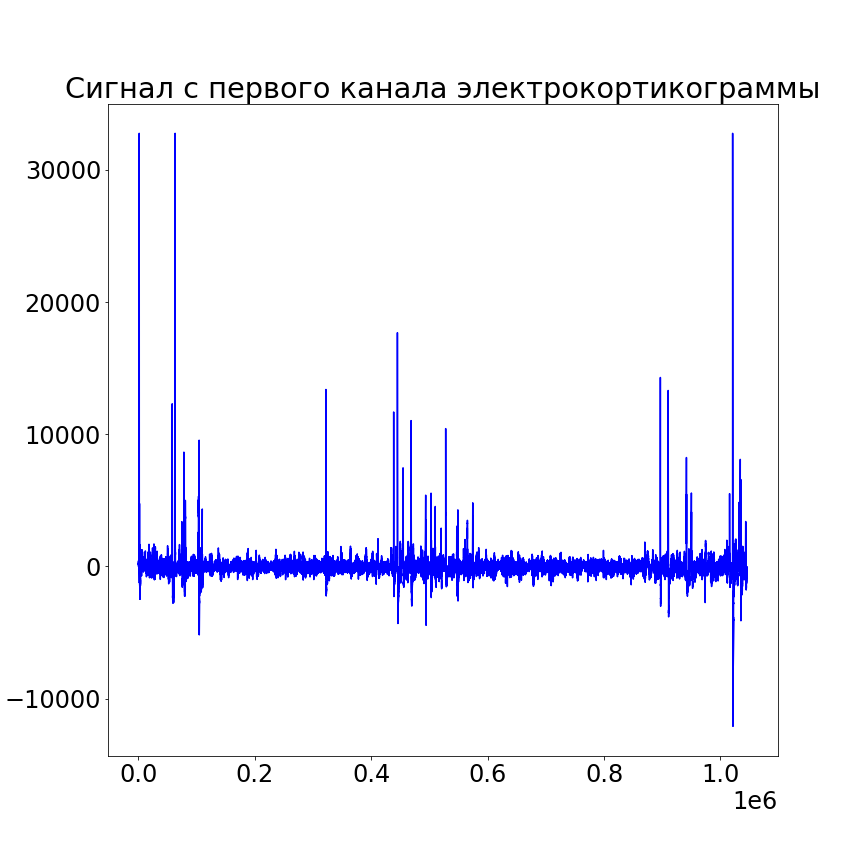
\includegraphics[width = 0.45\textwidth]{fig/Сигнал.eps}
     
\end{figure}
\begin{figure}[h]
    \centering
    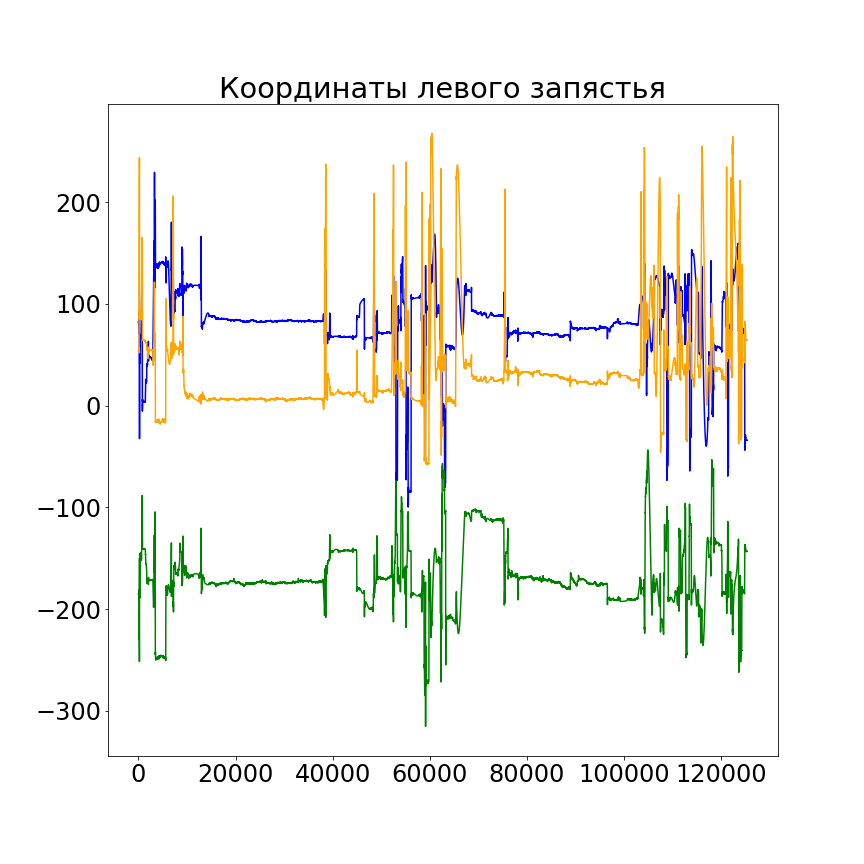
\includegraphics[width = 0.45\textwidth]{fig/Координаты.eps}
    \caption{Примеры временных рядов датасета.}
    \label{fig:example}
\end{figure}

\newpage
Для многомерного исходного ряда мультивекторные представления каждого из $64$ сигналов конкатенируются в признаковый вектор размерности $64 \times 6$, который используется для построения предсказания согласно разделу \ref{statement}. В качестве предсказательной модели используются линейные модели с регуляризаторами, полносвязные нейросети, рекуррентные нейросети и др.
\paragraph{}
Ниже приведём иллюстрации результатов решения задачи декодирования нейросетевой полносвязной моделью для двух значений ширины окна предыстории: $h = 10$ и $h = 25$. Архитектура выбранной сети предполагает пять внутренних слоёв с числом нейронов $512, 1024, 512, 256, 128$ соответственно, в качестве внутреннего критерия качества выбирается МАЕ. Отметим, что в данном эксперименте каждая из трёх координат каждого из сочленений предсказывалась независимо отдельной моделью. \paragraph{}
В качестве внешнего критерия оценки качества решения задачи используем коэффициент корреляции Пирсона между предсказанными и истинными значениями рядов на тестовой выборке:
$$ \text{corr} \Bigg( \hat{\textbf{Y}}_{t,p}, \textbf{Y}_{t,p} \Bigg)  = \frac{\text{cov} \Bigg( \hat{\textbf{Y}}_{t,p}, \textbf{Y}_{t,p} \Bigg)}{\sqrt{\text{cov} \Bigg( \textbf{Y}_{t,p}, \textbf{Y}_{t,p} \Bigg)} \sqrt{\text{cov} \Bigg( \hat{\textbf{Y}}_{t,p}, \hat{\textbf{Y}}_{t,p} \Bigg)}}$$
Значение коэффициента измеряется на кросс-валидации.

\paragraph{} 
Результаты сравнения решения для двух значений размерности предыстории представлены на рисунках ниже. В среднем удалось добиться коэффициента корреляции порядка $0.9$, что не уступает большинству методов решения задачи декодирования со снижением размерности в применении к даннму датасету.


\newpage

\begin{figure}[h!]
    \captionsetup{labelformat=empty}
    \centering
    \includegraphics[width = 1\textwidth]{fig/левое_плечо_10.eps}
\end{figure}

\begin{figure}[h]
    %\captionsetup{labelformat=empty}
    \centering
    \includegraphics[width = 1\textwidth]{fig/левое плечо_25.eps}
    \caption{Cверху: $h = 10$. Снизу: $h = 25$}
\end{figure}


\newpage

\vspace{3cm}

\begin{figure}[h]
    \captionsetup{labelformat=empty}
    \centering
    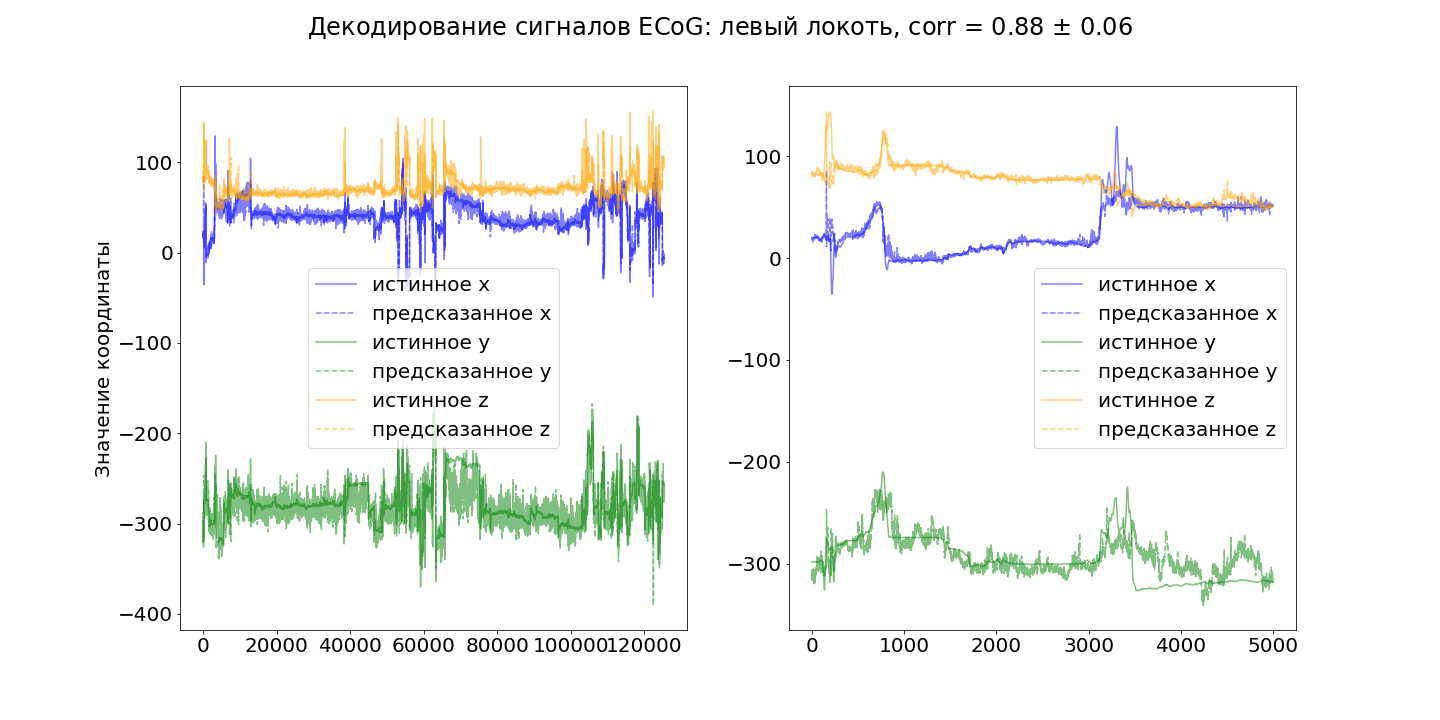
\includegraphics[width = 1\textwidth]{fig/левый локоть_10.eps}
\end{figure}

\begin{figure}[h]
    %\captionsetup{labelformat=empty}
    \centering
    \includegraphics[width = 1\textwidth]{fig/левый локоть_25.eps}
    \caption{Cверху: $h = 10$. Снизу: $h = 25$}
\end{figure}

\newpage

\begin{figure}[h]
    \captionsetup{labelformat=empty}
    \centering
    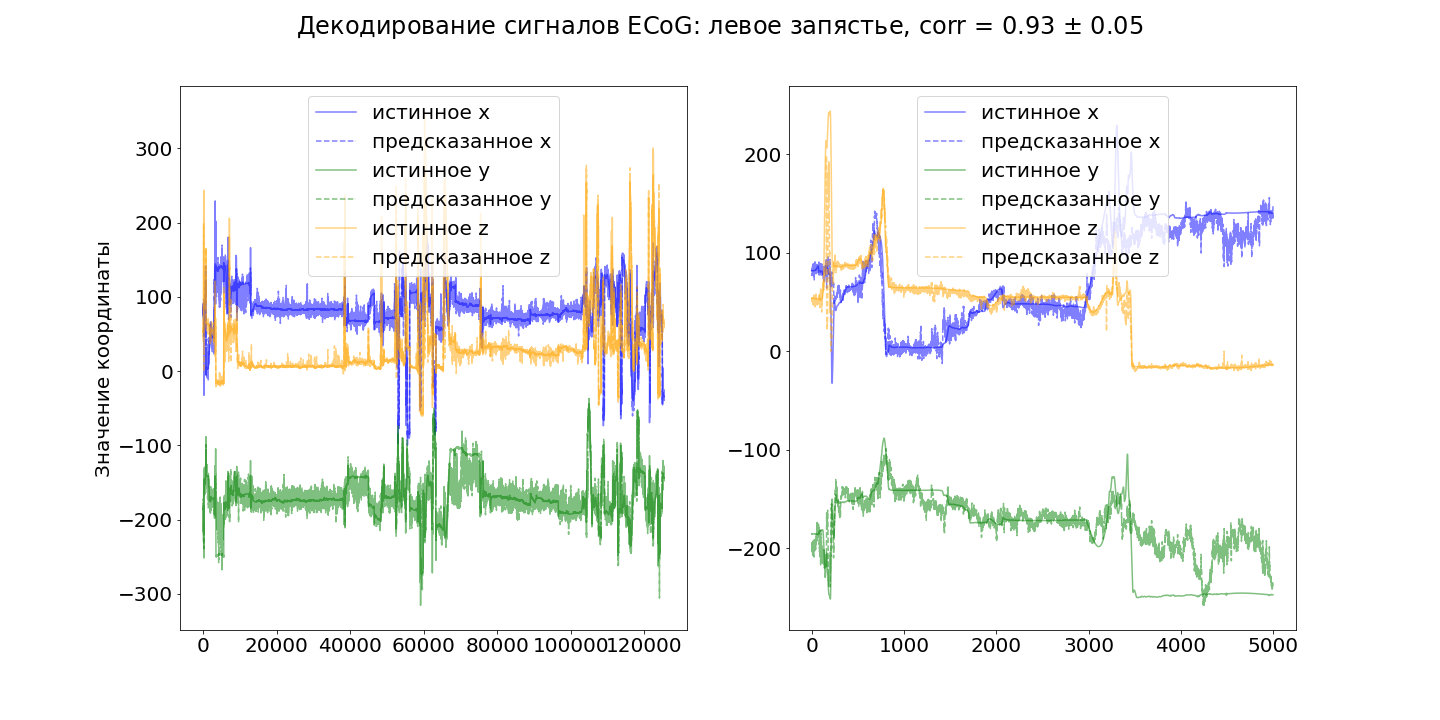
\includegraphics[width = 1\textwidth]{fig/левое запястье_10.eps}
\end{figure}

\begin{figure}[h]
    %\captionsetup{labelformat=empty}
    \centering
    \includegraphics[width = 1\textwidth]{fig/левое запястье_25.eps}
    \caption{Cверху: $h = 10$. Снизу: $h = 25$}
\end{figure}


%%%%%%%%%%%%%%%


\begin{comment}
\newpage

\begin{figure}[h]
    \captionsetup{labelformat=empty}
    \centering
    \includegraphics[width = 1\textwidth]{fig/правое_плечо_10.eps}
\end{figure}

\begin{figure}[h]
    %\captionsetup{labelformat=empty}
    \centering
    \includegraphics[width = 1\textwidth]{fig/правое_плечо_25.eps}
    \caption{Cверху: $h = 10$. Снизу: $h = 25$}
\end{figure}




\newpage


\begin{figure}[h]
    \captionsetup{labelformat=empty}
    \centering
    \includegraphics[width = 1\textwidth]{fig/правый_локоть_10.eps}
\end{figure}

\begin{figure}[h]
    %\captionsetup{labelformat=empty}
    \centering
    \includegraphics[width = 1\textwidth]{fig/правый_локоть_25.eps}
    \caption{Cверху: $h = 10$. Снизу: $h = 25$}
\end{figure}


\newpage

\begin{figure}[h]
    \captionsetup{labelformat=empty}
    \centering
    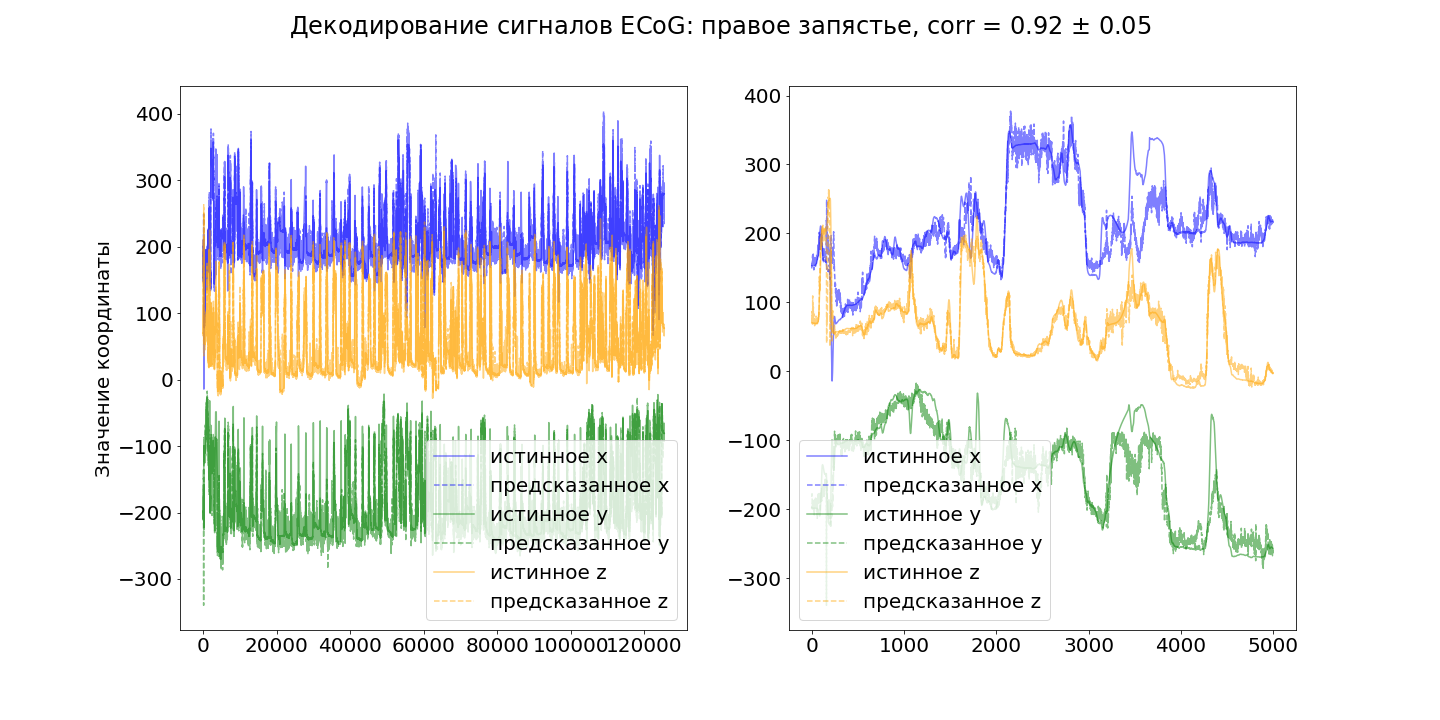
\includegraphics[width = 1\textwidth]{fig/правое запястье_10.eps}
\end{figure}

\begin{figure}[h]
    %\captionsetup{labelformat=empty}
    \centering
    \includegraphics[width = 1\textwidth]{fig/правое запястье_25.eps}
    \caption{Cверху: $h = 10$. Снизу: $h = 25$}
\end{figure}
\end{comment}

\newpage
\section*{Заключение}
\addcontentsline{toc}{section}{\protect\numberline{}Заключение}

Предложен нелинейный метод снижения размерности в задаче декодирования сигналов, позволяющий построить информативное шестимерное представление элемента фазовой траектории исходного сигнала в виде мультивектора. В методе формируется пространственно-временное представление отрезка временного ряда в виде графа в трёхмерном пространстве, узлы которого затем погружается в конформную геометрическую алгебру. Применение метода позволило восстановить траектории движения конечностей обезьяны по сигналам электрокортиграммы головного мозга, качество восстановления не уступает альтернативным методам при гораздо большей степени сжатия данных. Дальнейшее развитие работы подразумевает изучение свойств полученных мультивекторных описаний рядов под действием операторов алгебры, отказ от предопределённой пространственной конфигурации представления и подробное исследование качества решения задачи декодирования в зависимости от структурных параметров метода.


\newpage
\addcontentsline{toc}{section}{\protect\numberline{}Список литературы}
\bibliographystyle{unsrt}
\bibliography{GA_references}





\end{document} 
